\documentclass[12pt,a4paper]{scrartcl}

%========================================================================================
%SPRACHE

\usepackage[ngerman]{babel} 
\usepackage[T1]{fontenc} 				% richtige Silbentrennung
\usepackage[utf8]{inputenc}
%========================================================================================
%DARSTELLUNG

\usepackage[small,compact]{titlesec} 		% Verkleinerung von Section-Ueberschriften
\usepackage{graphicx}				  	% Einbinden von Graphiken .ps, .pdf, .png

\usepackage{amsmath}					% mathematische Symbole
\usepackage {ulem} 						%\emph{Text}: Text wird unterstrichen
\setlength{\parindent}{0pt}				% Zeile nach Absatz einruecken 1pt oder nicht 0pt.

\usepackage{float} % alles möglichen Sachen mit [h] an die richtige Stelle zwingen
%========================================================================================
%FARBEN

\usepackage[usenames,dvipsnames]{color}	

									%Apricot 	Aquamarine 	Bittersweet 	Black
									%Blue 	BlueGreen 	BlueViolet 	BrickRed
									%Brown 	BurntOrange 	CadetBlue 	CarnationPink
									%Cerulean 	CornflowerBlue 	Cyan 	Dandelion
									%DarkOrchid 	Emerald 	ForestGreen 	Fuchsia
									%Goldenrod 	Gray 	Green 	GreenYellow
									%JungleGreen 	Lavender 	LimeGreen 	Magenta
									%Mahogany 	Maroon 	Melon 	MidnightBlue
									%Mulberry 	NavyBlue 	OliveGreen 	Orange
									%OrangeRed 	Orchid 	Peach 	Periwinkle
									%PineGreen 	Plum 	ProcessBlue 	Purple
									%RawSienna 	Red 	RedOrange 	RedViolet
									%Rhodamine 	RoyalBlue 	RoyalPurple 	RubineRed
									%Salmon 	SeaGreen 	Sepia 	SkyBlue
									%SpringGreen 	Tan 	TealBlue 	Thistle
									%Turquoise 	Violet 	VioletRed 	White
									%WildStrawberry 	Yellow 	YellowGreen 	YellowOrange
									
									% verwenden mit: 
									% \pagecolor{declared-color}
									% {\color{declared-color} text}
									% \colorbox{declared-color1}{\color{declared-color2} text}

									%========================================================================================
%Zur Einbindung von Programmiertexten mit:
				% \begin{lstlisting}
				%put your code here
				%\end{lstlisting}
				
\usepackage{listings}
\lstset{ %
language=bash,                			% the language of the code
basicstyle=\footnotesize,       			% the size of the fonts that are used for the code
numbers=left,                   				% where to put the line-numbers
numberstyle=\footnotesize,      			% the size of the fonts that are used for the line-numbers
stepnumber=2,                   				% the step between two line-numbers. If it's 1, each line 
                                					% will be numbered
numbersep=5pt,                  			% how far the line-numbers are from the code
backgroundcolor=\color{white},  		% choose the background color. You must add \usepackage{color}
showspaces=false,               			% show spaces adding particular underscores
showstringspaces=false,        		 	% underline spaces within strings
showtabs=false,                 				% show tabs within strings adding particular underscores
frame=single,                   				% adds a frame around the code
tabsize=2,                      				% sets default tabsize to 2 spaces
captionpos=b,                   				% sets the caption-position to bottom
breaklines=true,                				% sets automatic line breaking
breakatwhitespace=false,        			% sets if automatic breaks should only happen at whitespace
title=\lstname,                 				% show the filename of files included with \lstinputlisting;
                                					% also try caption instead of title
}
%========================================================================================


%LOAD FANCYHDR fuer Kopf- und Fu{ß}zeilen
\usepackage{fancyhdr}					% Paket laden	für einfache Handhabung von Kopf-und Fu{ß}zeile
\pagestyle{fancy}							
\fancyhf{}
\fancyhead[L]{\small{\textbf{Potentialtheorie \\ Semesterabschlussarbeit}}}
\fancyhead[R]{\small{Sebastian Beyer \\ 25. Februar 2013}}
\fancyfoot[C]{\thepage} 			%Seitennummer



\usepackage{subfigure}

\addto\captionsngerman{
\renewcommand{\figurename}{Abb.}
\renewcommand{\tablename}{Tab.}
}

\usepackage{booktabs}




\begin{document}


\section*{Gravimetrische Modellierung eines vulkanischen Förderschlotes}

\subsection*{Einleitung}

In dieser Arbeit untersuche ich die Detektierbarkeit eines vulkanischen Förderschlotes per Gravimetrie.

Dazu nutze ich das bereits in der Übung entwickelte Programm um eine Magmakammer gravimetrisch zu modellieren.
Es implementiert den Algorithmus von Donald Plouff\footnote{Donald Plouff, Gravity and magnetic fields of polygonal prisms and application to magnetic terrain corrections, August 1976, Geophysics 41 4 p.727-741}, um die Schwerewirkung beliebig geformter Körper zu berechnen.\\

Magmakammern bilden sich in der Lithospähre, wenn flüssiges Magma in Form von Blasen aus tieferen Bereichen aufgrund seiner geringeren Dichte aufsteigt und sich dort sammelt, wo die Dichte ähnlich groß wie die des umgebenden Gesteins ist.

Dort kann es zu spontanen Entgasungen kommen, wodurch die Dichte weiter abnimmt und das Material aufsteigt. 
Es bildet sich ein Vulkanschlot, welcher bis an die Oberfläche vordringen kann.\\

Die Dichteuntersschiede lassen sich durch Gravimetrische Messungen feststellen und können möglicherweise Helfen, entsprechende Strukturen frühzeitig zu entdecken.

\clearpage
\section*{Geometrie}

\begin{figure}[htb]
\centering
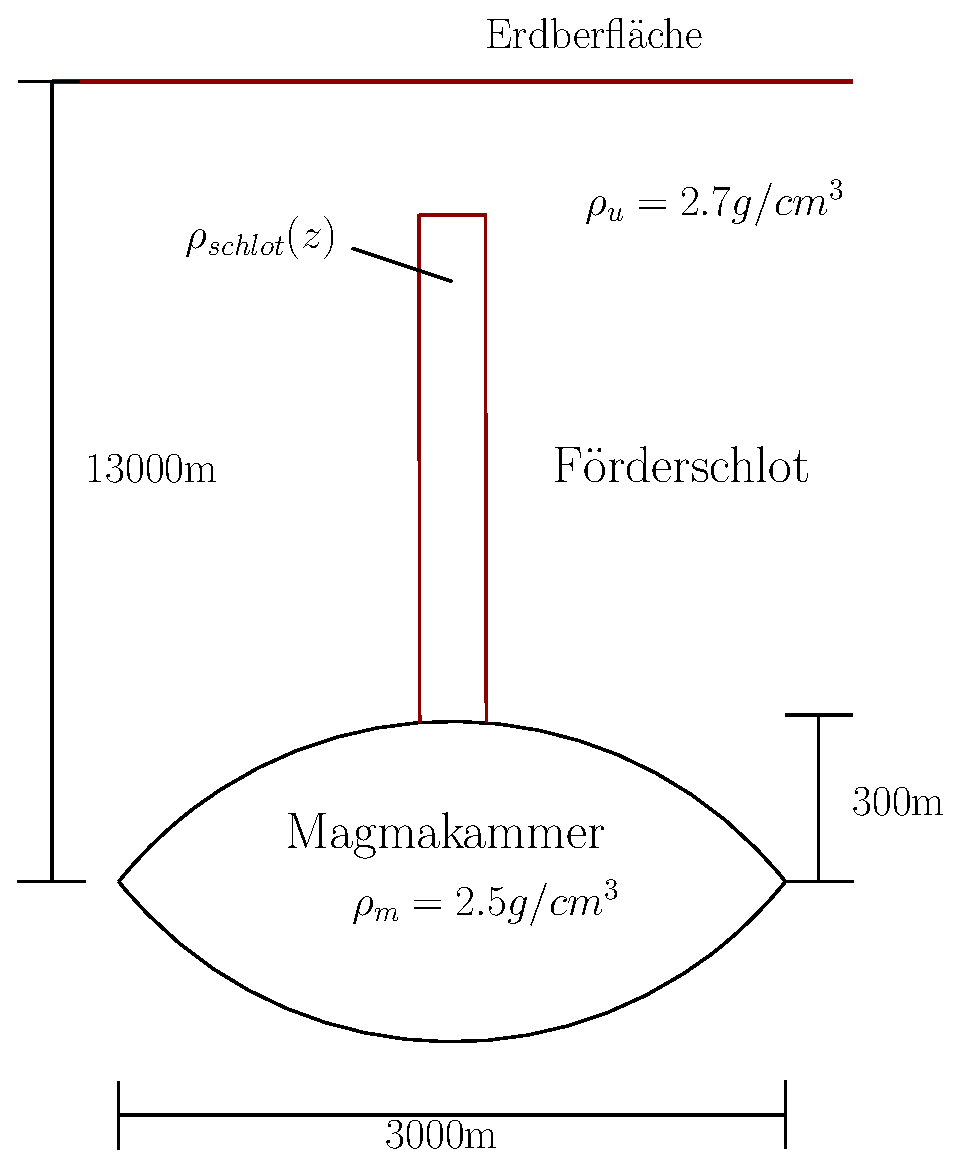
\includegraphics[width=0.4\textwidth]{../figures/geometry}
\caption{Geometrie des Modells}
\label{geometry}
\end{figure}


In Abbildung \ref{geometry} ist die verwendete Modellgeometrie dargestellt.

Ich möchte eine relativ tief gelegene Magmakammer in 13 Kilometern Tiefe modellieren, welche ich als Ellipsoid mit einer Dichte von $2.5g/cm^3$ annähre. Die kurze Halbachse ist 300m lang, die lange Halbachse 1500m.

Das umgebende Gestein erhält die durchschnittliche Krustengesteinsdichte von $2.7g/cm^3$.\\

Im Schlot nimmt die Dichte wie bereits erwähnt nach oben hin ab. Beschrieben ist dies z.B. bei Kazahaya\footnote{
Kohei Kazahaya, Hiroshi Shinohara, and Genji Saito, 2002, Degassing process of Satsuma-Iwojima volcano, Japan: Supply of volatile components from a deep magma chamber,Geological Survey of Japan, AIST, 1-1-1 Higashi Tsukuba, Ibaraki 305-8567, Japan
}. Daher entstammt auch Abbildung \ref{origdens}, welche die Abhängigkeit der Dichte vom Umgebungsdruck und damit der Tiefe darstellt.\\

\begin{figure}[htb]
\centering
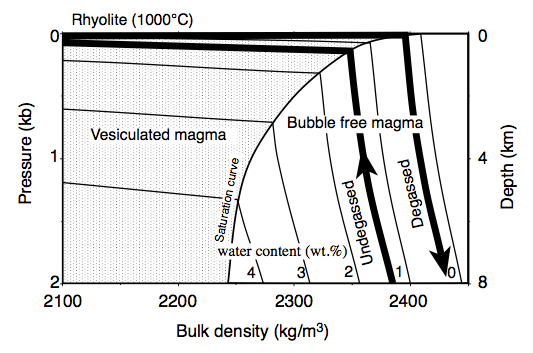
\includegraphics[width=0.6\textwidth]{../figures/origdens.png}
\caption{Dichteverteilung in einem Schlot nach Kazahaya et al 2002}
\label{origdens}
\end{figure}

\clearpage
Da eine genaue Berechnung der Dichteabnahme sehr kompliziert ist und den Rahmen dieser Arbeit sprengen würde, habe ich den Dichteverlauf vereinfacht als linear angenommen.
In Abbildung \ref{rhomodel} ist die Abhängigkeit zu erkennen. Dabei habe ich den Vulkanschlot in 10 Ebenen unterteilt, welchen jeweils eine Dichte zugewiesen wird.

Es ist er Dichteunterschied $\Delta \rho$ dargestellt, da dieser vom Programm verwendet wird, um Anomalien zu berechnen.

\begin{figure}[htb]
\centering
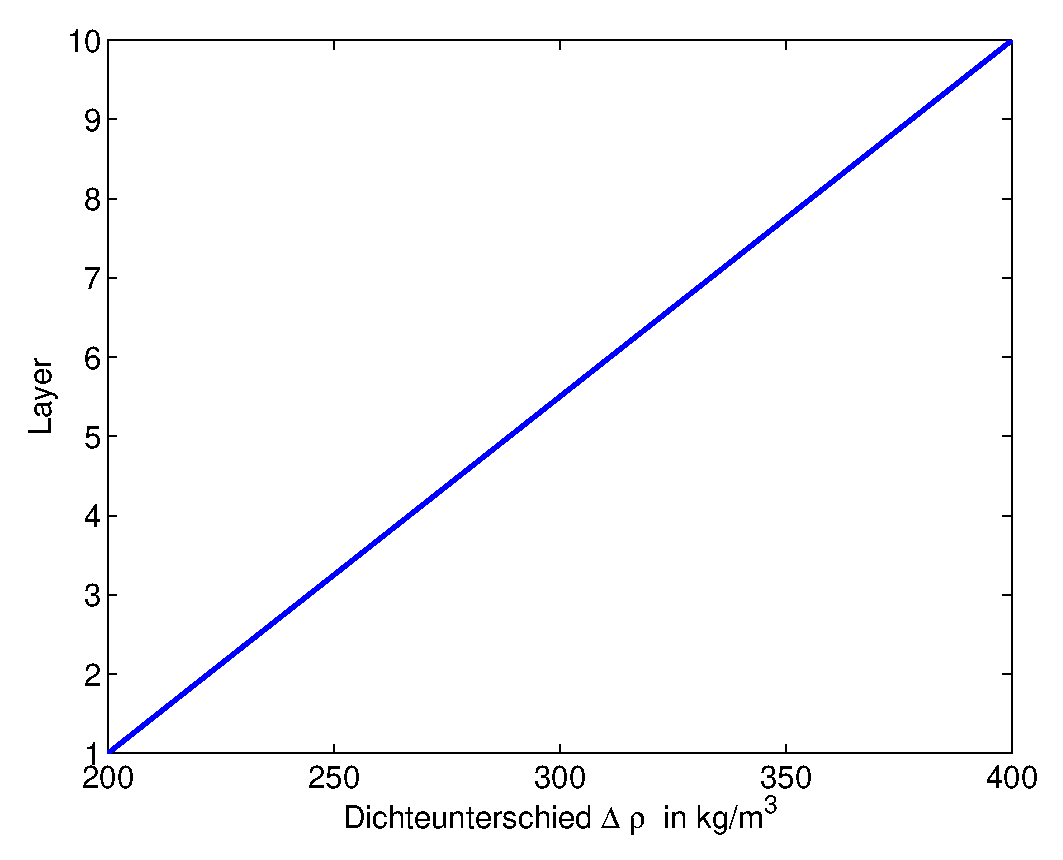
\includegraphics[width=0.6\textwidth]{../figures/rho_model}
\caption{Vereinfachtes, lineares Dichtemodell}
\label{rhomodel}
\end{figure}


\subsection*{Programmaufbau}



\subsection*{Ergebnisse}

\begin{figure}[htb]
\centering
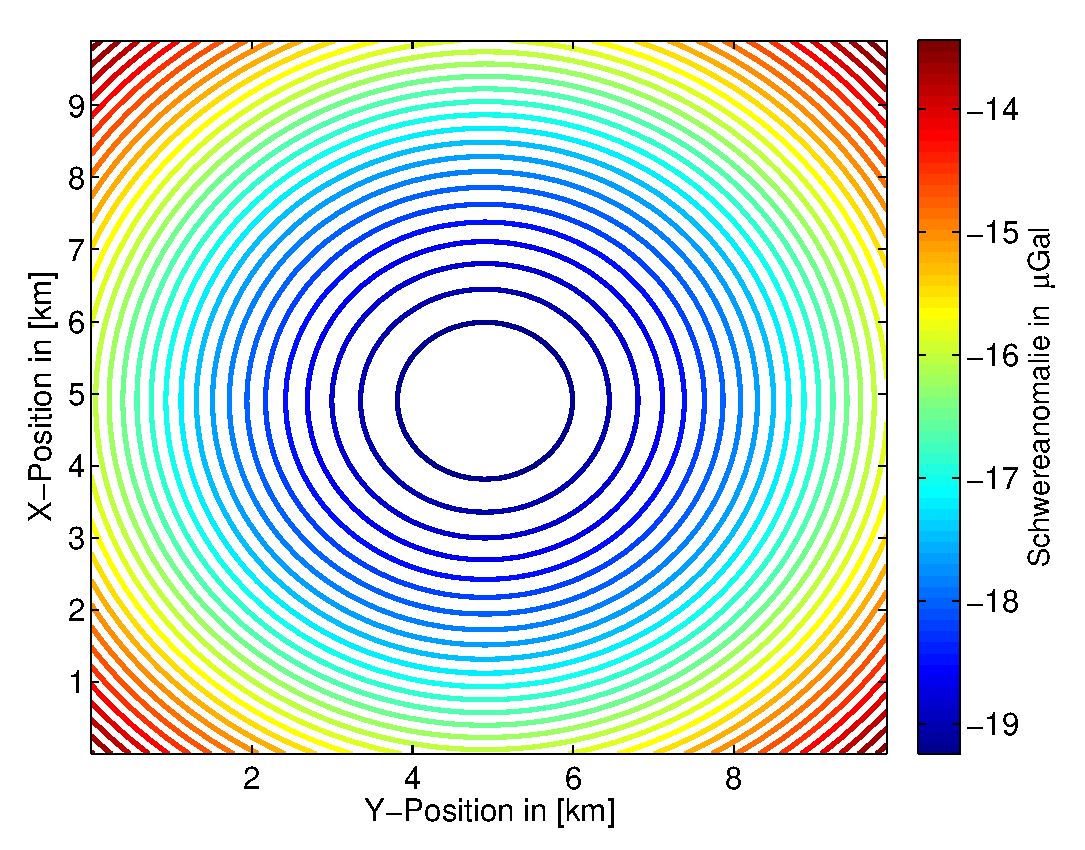
\includegraphics[width=0.8\textwidth]{../figures/2dchamber_contour}
\caption{2dchamber}
\label{2dchamber}
\end{figure}


\begin{figure}[htb]
\centering
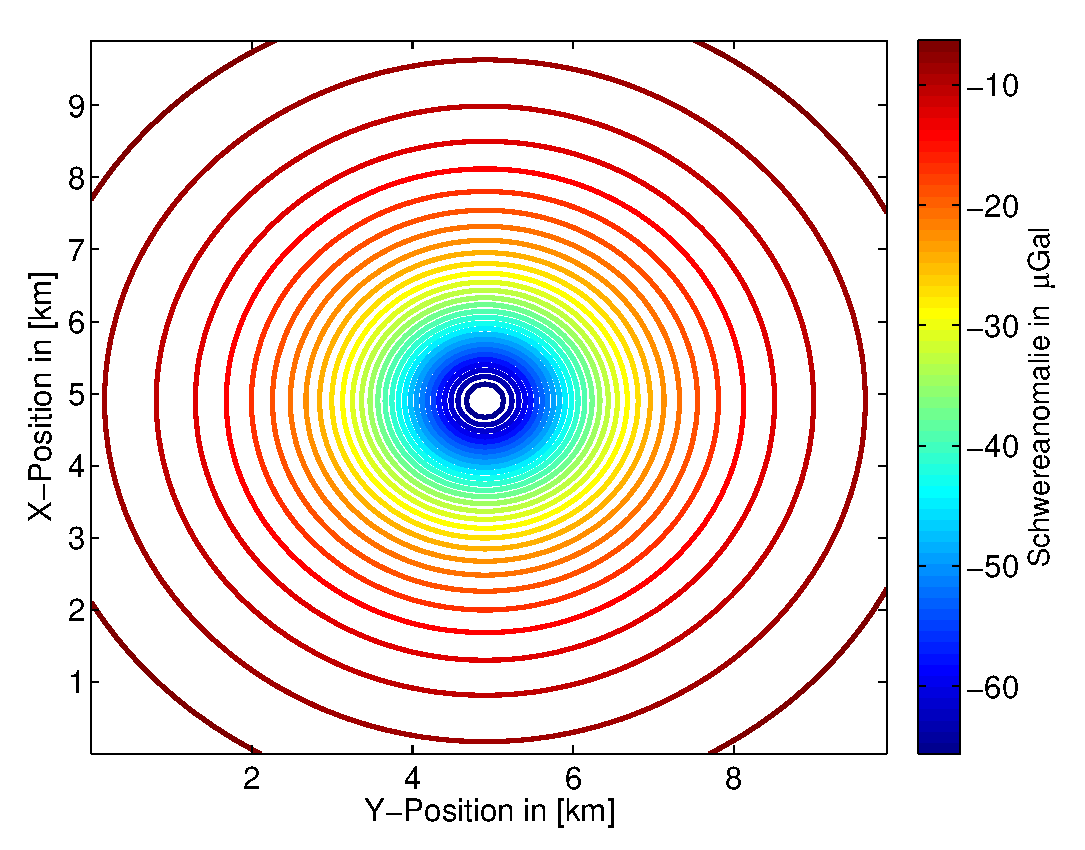
\includegraphics[width=0.8\textwidth]{../figures/2dconduit_contour}
\caption{2dconduit}
\label{2dconduit}
\end{figure}

\begin{figure}[htb]
\centering
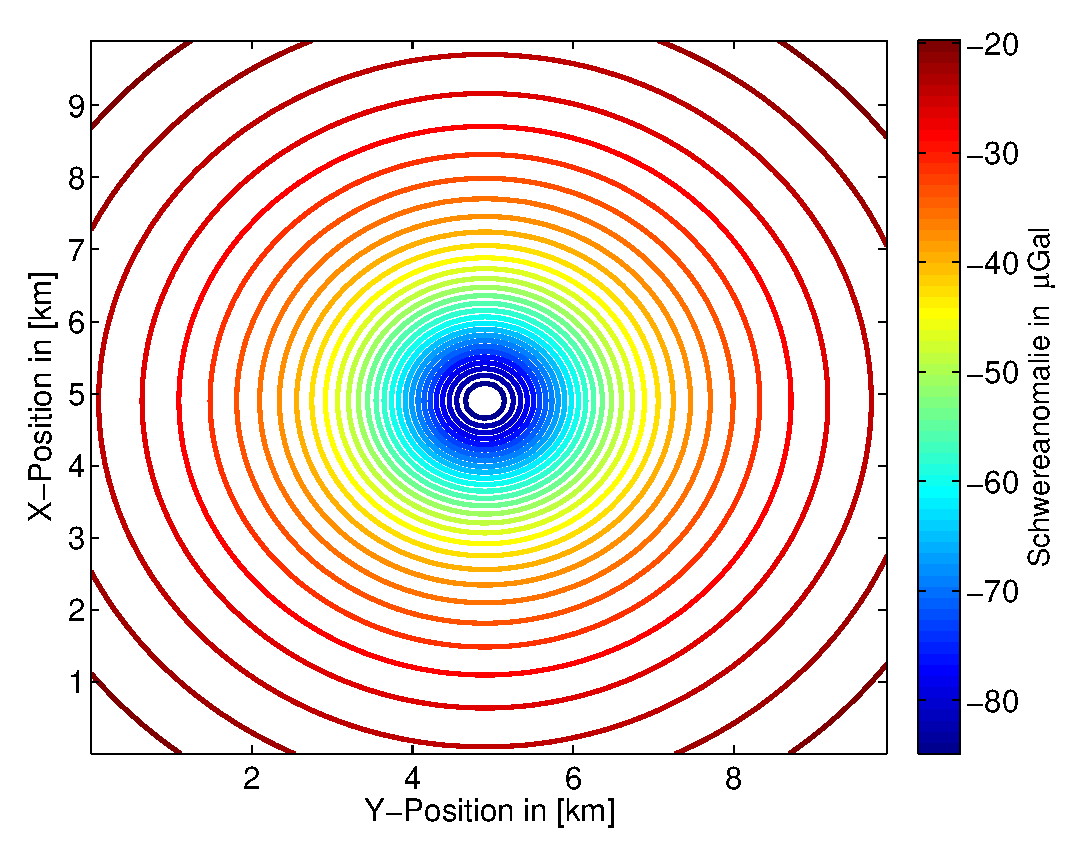
\includegraphics[width=0.8\textwidth]{../figures/2dwhole_contour}
\caption{2dwhole}
\label{2dwhole}
\end{figure}

\begin{figure}[htb]
\centering
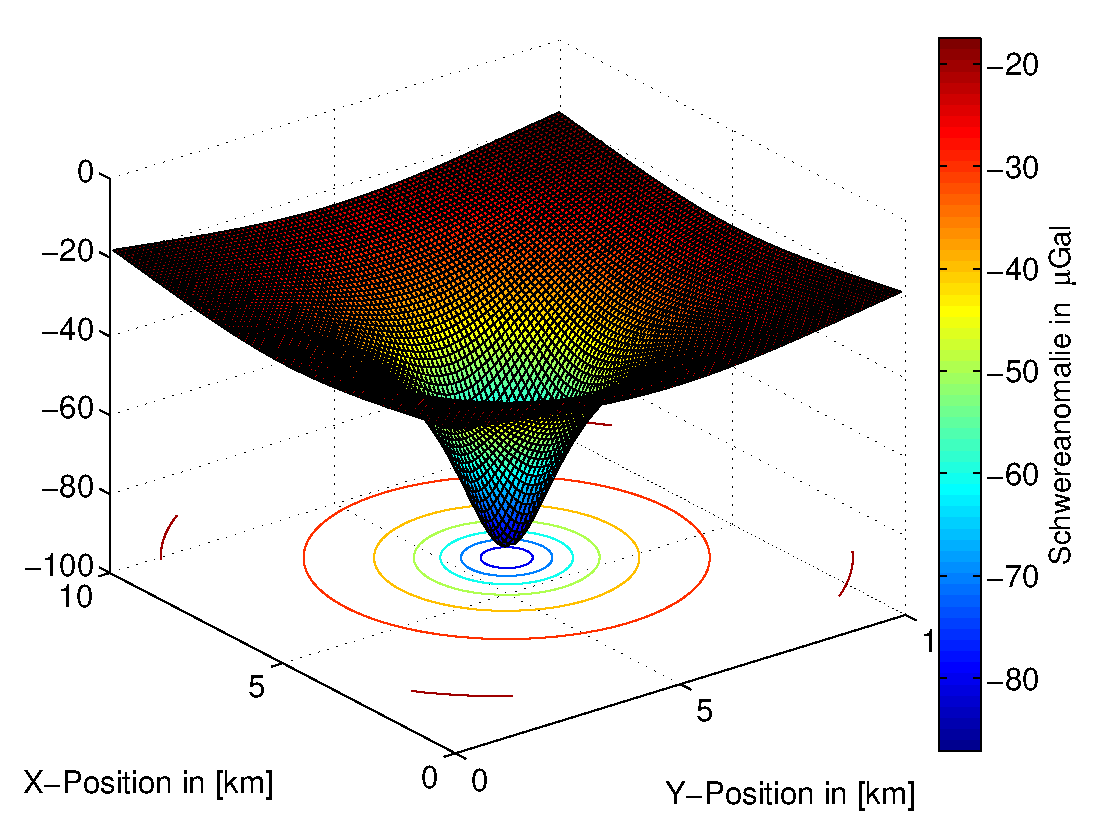
\includegraphics[width=0.8\textwidth]{../figures/2dwhole_surfc}
\caption{2dsurfc}
\label{2dsurfc}
\end{figure}


\begin{figure}[htb]
\centering
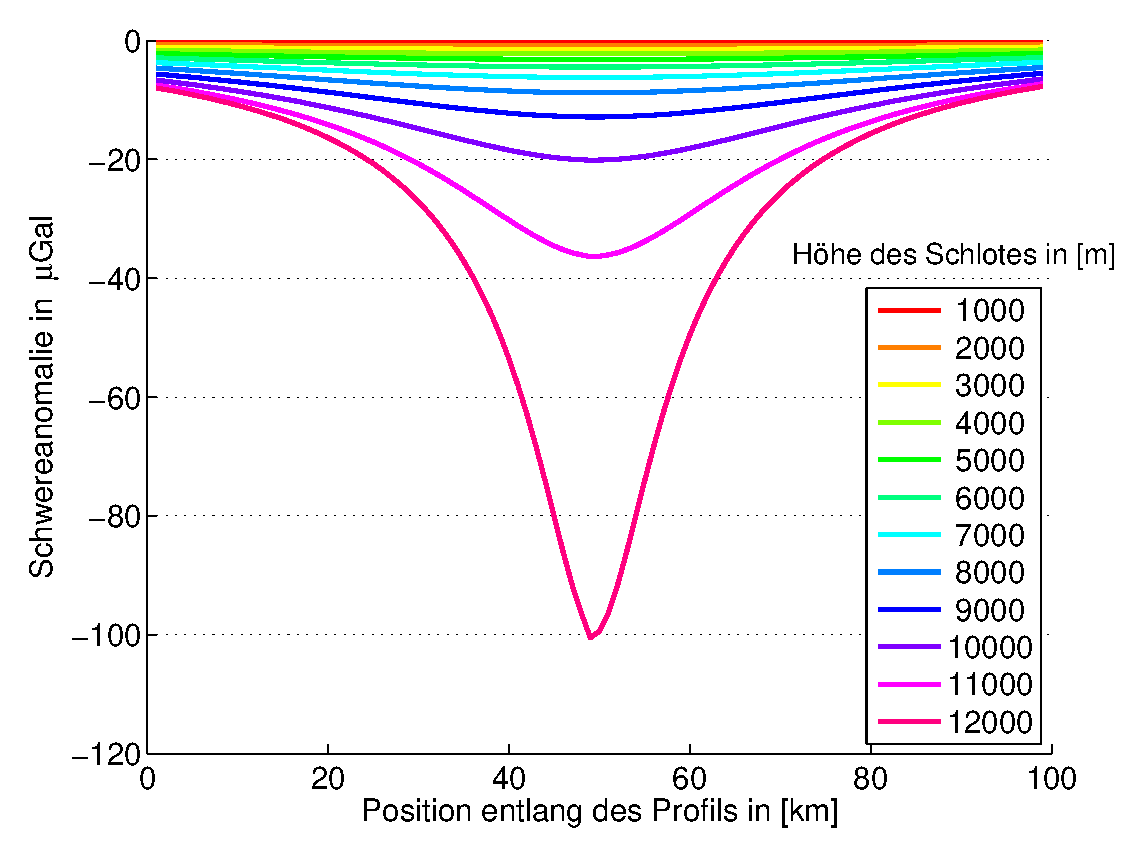
\includegraphics[width=0.8\textwidth]{../figures/var_height}
\caption{variation of height}
\label{varheight}
\end{figure}




\end{document}



